%******************************************************************************
% KOMA-Script article scrartcl
%******************************************************************************
\documentclass[10pt, b5paper]{article} 

% Add here all the packages that will be used in the document
%******************************************************************************
% Packages 
%******************************************************************************
% For hyperlinks 
\usepackage{url}

% Add no chapters to the article 
\usepackage[nochapters]{classicthesis}

% Setup the page geometry
\usepackage{geometry}
\geometry{a4paper, total={210mm, 297mm}, 
left=20mm, right=20mm, top=20mm, bottom=20mm}

% Use tikz to add watermarks to the document
\usepackage{blindtext,tikz}
\usetikzlibrary{calc}

% Use the classicthesis style for the style of the document
\usepackage[nochapters]{classicthesis} 

% Use the currvita style for the layout of the document
\usepackage[LabelsAligned]{currvita} 

% Required for adding links	and customizing them
\usepackage{hyperref} 

 % Set link colors
\hypersetup{colorlinks, breaklinks, urlcolor=Maroon, linkcolor=Maroon}


% Add a list of new commands 
%******************************************************************************
% Commands 
%******************************************************************************
\newcommand{\latex}{\LaTeX\xspace}
\newcommand{\tex}{\TeX\xspace}

\usepackage{listings}
\usepackage{color}
\usepackage{graphicx}
\usepackage{caption}
\usepackage{subcaption}

\graphicspath{{images/report3/}}

\definecolor{dkgreen}{rgb}{0,0.6,0}
\definecolor{gray}{rgb}{0.5,0.5,0.5}
\definecolor{mauve}{rgb}{0.58,0,0.82}

\lstset{frame=tb,
  language=Java,
  aboveskip=3mm,
  belowskip=3mm,
  showstringspaces=false,
  columns=flexible,
  basicstyle={\small\ttfamily},
  numbers=none,
  numberstyle=\tiny\color{gray},
  keywordstyle=\color{blue},
  commentstyle=\color{dkgreen},
  stringstyle=\color{mauve},
  breaklines=true,
  breakatwhitespace=true,
  tabsize=3
}

%******************************************************************************
% DOCUMENT STARTS HERE 
%******************************************************************************
\begin{document}

% TITLE 
\title{\rmfamily\normalfont\spacedallcaps{
Report \#{3}
}}

% PROJECT NAME -> ADD YOUR PROJECT NAME HERE
\author{{\small Automatic Mandible Segmentation Using VTK}}

% AUTOMATIC DATE -> DON'T CHANGE MANUALLY
\date{\footnotesize{\today}}

% MAKE THE TITLE -> DON'T CHANGE MANUALLY
\maketitle

% DON'T INCLUDE THE ABSTRACT FOR THE MOMENT
% % \begin{abstract}
% \noindent Abstract
% \end{abstract}
 
%******************************************************************************
% TABLE OF CONTENTS (uncomment to show / comment to hide)
%******************************************************************************     
% \tableofcontents


%******************************************************************************
% Report Content
%******************************************************************************
\section{Report Details}
\begin{center}
\begin{tabular}{ l | c }
\hline 
Report ID & 3  \\ % Change the sprint ID here 
\hline 
Report Duration & 2 Week \\ % Change the duration here 
\hline 
Beginning & 31.10.2016 \\ % Change the start data here
\hline 
End & 15.11.2016 \\ % Change the end data here
\hline 
\end{tabular}
\end{center}

%\section{Objectives}
\section{Original Objectives}
\begin{enumerate}
\item Thresholding Implementation.
\item Implementing mandible Segmentation Algorithm.
\item Filtering the Data.
\item GUI Design.
\end{enumerate}

\section{Accomplished Objectives}
\subsection{Thresholding Implementation}
figure \ref{fig:Thresholding} shows the result of applying thresholding on the volume of interest with different values of threshold, It is clear that at 1100 the skin still appears, for 1200 it is better but still some of soft tissues appears, at 1400 almost all soft tissues are suppressed and only bone appears. Applying Thresholding is done in parallel using OpenMP compiler directives, as the domain or data decomposition is valid at this stage. The running time for thresholding is at most 2 seconds.

\begin{figure}
    \centering
    \begin{subfigure}[b]{0.33\textwidth}
        \centering
        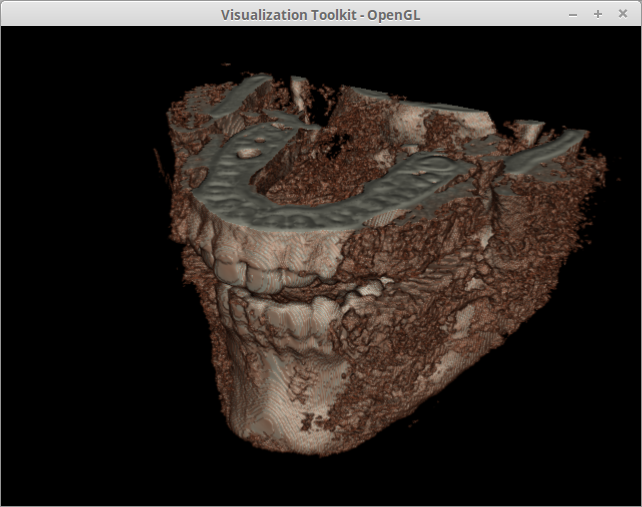
\includegraphics[width=\textwidth]{T1100}
        \caption{Threshold is 1100.}
    \end{subfigure}
    \hfill
    \begin{subfigure}[b]{0.33\textwidth}
        \centering
        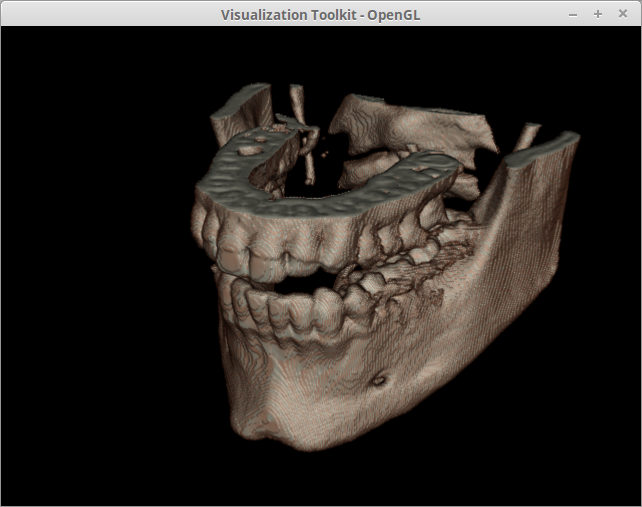
\includegraphics[width=\textwidth]{T1200}
        \caption{Threshold is 1200}
    \end{subfigure}
      \hfill
    \begin{subfigure}[b]{0.33\textwidth}
        \centering
        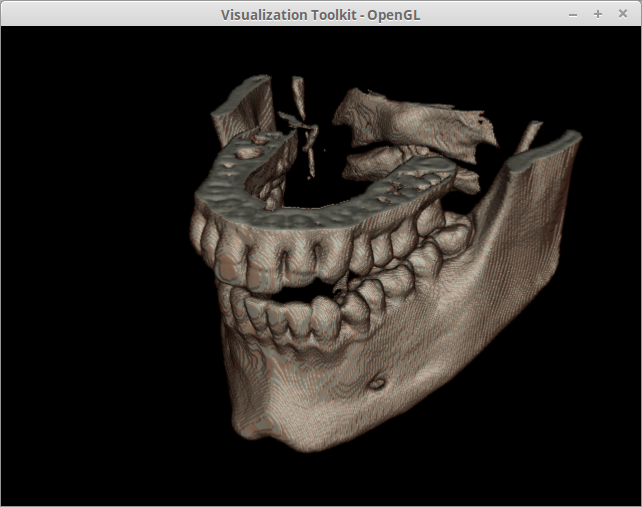
\includegraphics[width=\textwidth]{T1400}
        \caption{Threshold is 1400}
    \end{subfigure}
    \caption{Applying Thresholding for different thresholds}
    \label{fig:Thresholding}
\end{figure}

\subsection{Implementing Mandible Segmentation Algorithm}
For mandible segmentation Thresholding algorithm using labeling and connectivity is applied, The connectivity of data point is checked with its 13th neighbourhood, 9 at the previous slice and 4 at the same slice, if the point is connected to a labled point so it will have the same label, and if it is not have any labeled data point in its neighbours, it will be a new segment with a new label. mapping id of  each none zero data point to its label is maintained using a \textit{std::unordered\_map} that implements hash table based map with more time efficiency in restoring data from its key. on the other hand a segments list is constructed to maintain the count of points connected to each segment and a set of segments equivalent to this segment.

After labeling all none zero data points, we have to get the largest segment. by adding the count of points of each connected segments to each segment, then we get the total points of each segment and then we select the largest one. The more challenging task is to acquire all connected segments of the largest segment from its connected segments Set, it is solved efficiently using Breadth First Search Algorithm to traverse all nodes of connected segments tree. 

Figure \ref{fig:BS} shows different views of the volume after extracting volume of interest and applying thresholding and before applying segmentation algorithm, figure \ref{fig:RC}, \ref{fig:MC} show the results of segmentation, figure \ref{fig:RC} shows the  mandible rendered using ray casting and figure \ref{fig:MC} using marching cubes. The running time of segmentation algorithm has been enhanced after applying Breadth First Algorithm, as it was about  3 minutes and now it is only 30 seconds of 512 x 512 x 525 volume. 

\begin{figure}
    \centering
    \begin{subfigure}[b]{0.33\textwidth}
        \centering
        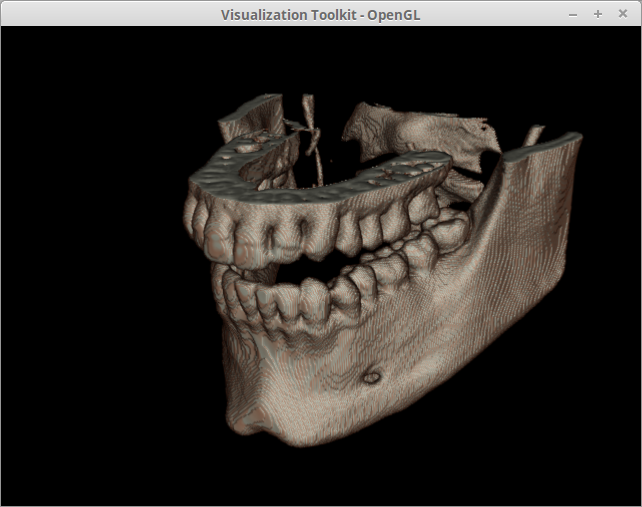
\includegraphics[width=\textwidth]{BSS}
        \caption{Side View of Volume}
    \end{subfigure}
    \hfill
    \begin{subfigure}[b]{0.33\textwidth}
        \centering
        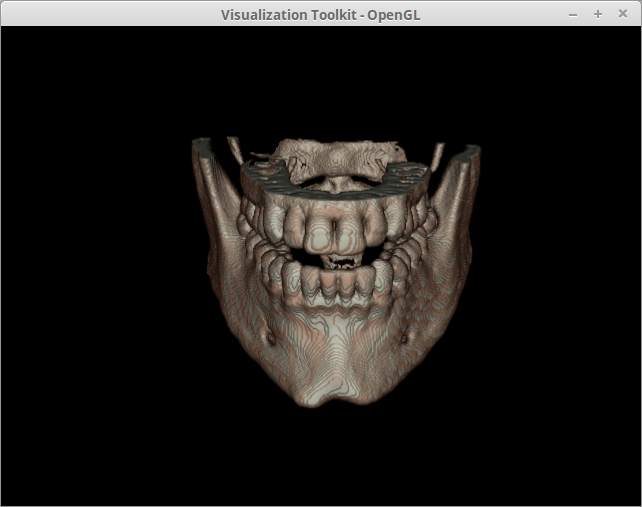
\includegraphics[width=\textwidth]{BSF}
        \caption{Front View of Volume}
    \end{subfigure}
      \hfill
    \begin{subfigure}[b]{0.33\textwidth}
        \centering
        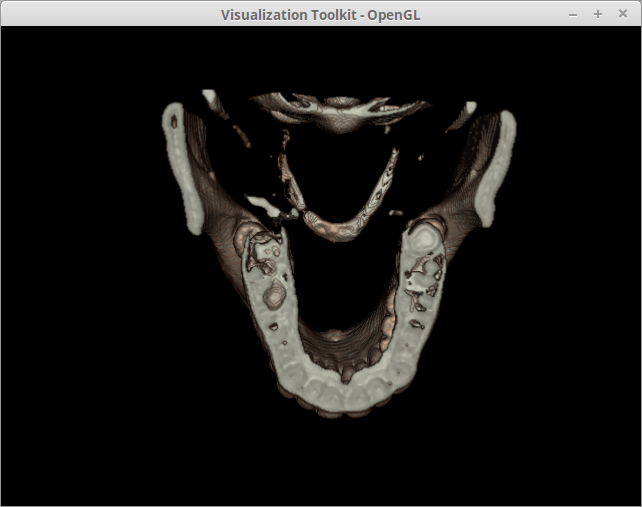
\includegraphics[width=\textwidth]{BST}
        \caption{Top View of Volume}
    \end{subfigure}
    \caption{Volume of Interest Before Segmentation with different Views}
    \label{fig:BS}
\end{figure}


\begin{figure}
    \centering
    \begin{subfigure}[b]{0.33\textwidth}
        \centering
        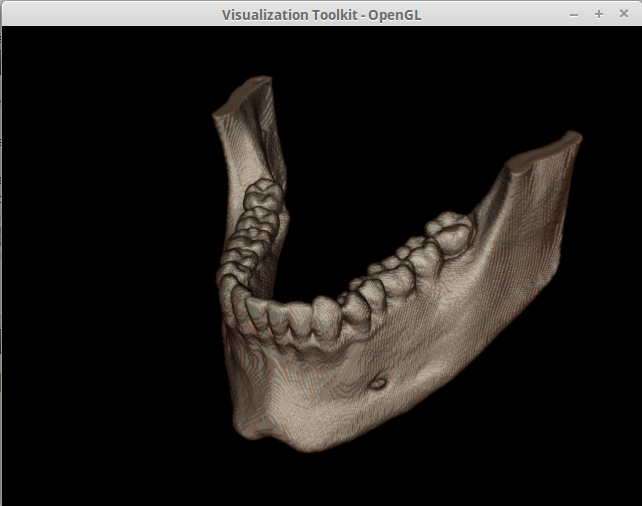
\includegraphics[width=\textwidth]{RCS}
        \caption{Side View of Volume}
    \end{subfigure}
    \hfill
    \begin{subfigure}[b]{0.33\textwidth}
        \centering
        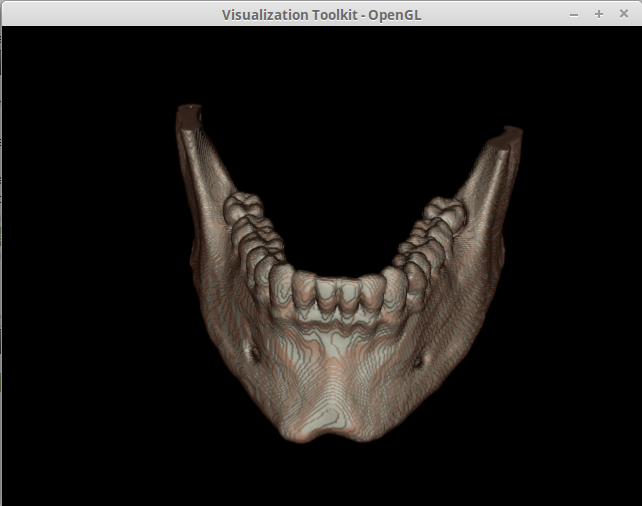
\includegraphics[width=\textwidth]{RCF}
        \caption{Front View of Volume}
    \end{subfigure}
      \hfill
    \begin{subfigure}[b]{0.33\textwidth}
        \centering
        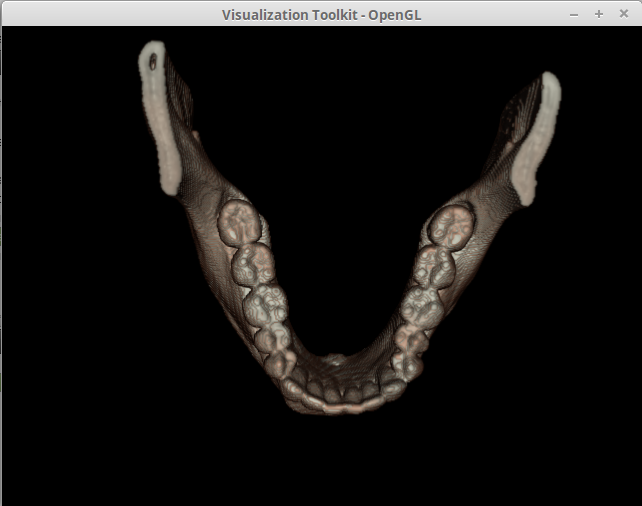
\includegraphics[width=\textwidth]{RCT}
        \caption{Top View of Volume}
    \end{subfigure}
    \caption{Rendering of Volume After Segmentation with different Views using  Ray Casting rendering technique.}
    \label{fig:RC}
\end{figure}

\begin{figure}
    \centering
    \begin{subfigure}[b]{0.33\textwidth}
        \centering
        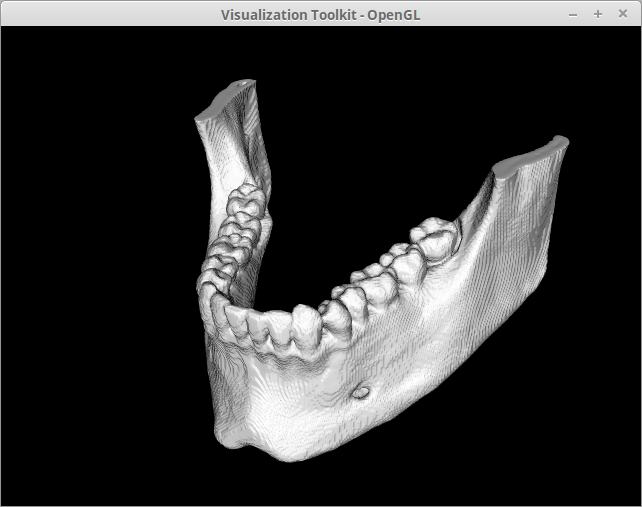
\includegraphics[width=\textwidth]{MCS}
        \caption{Side View of Volume}
    \end{subfigure}
    \hfill
    \begin{subfigure}[b]{0.33\textwidth}
        \centering
        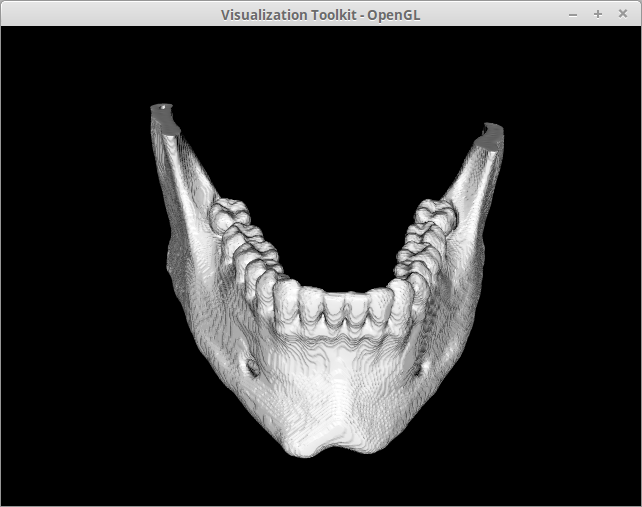
\includegraphics[width=\textwidth]{MCF}
        \caption{Front View of Volume}
    \end{subfigure}
      \hfill
    \begin{subfigure}[b]{0.33\textwidth}
        \centering
        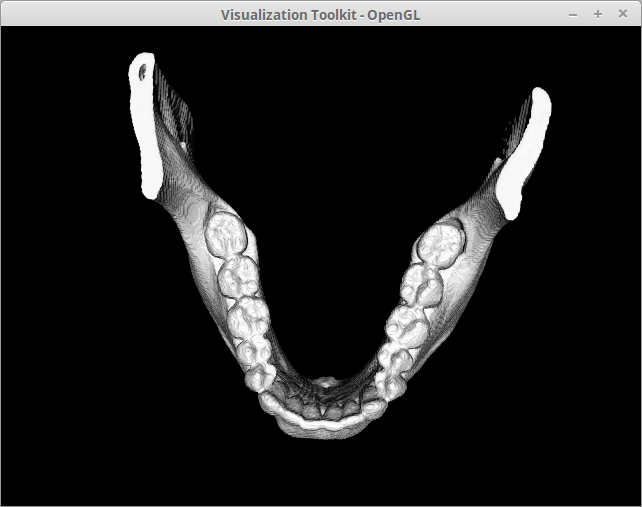
\includegraphics[width=\textwidth]{MCT}
        \caption{Top View of Volume}
    \end{subfigure}
    \caption{Rendering of Volume After Segmentation with different Views using  Marching Cubes rendering technique.}
    \label{fig:MC}
\end{figure}

\section{Missed Objectives}

\begin{itemize}
\item Filtering the Data.
\item GUI Designe
\end{itemize}

\section{Next Step}
\begin{itemize}
\item Filtering data to remove noise.
\item Graphical user interface design.
\item Enhance framework and more code optimization.
\item Writing a short paper.
\end{itemize}   
    
%******************************************************************************
% DOCUMENT ENDS HERE 
%******************************************************************************
\end{document}